\section{Bringing Topologies to Life---Emulating Nodes and Links}
\label{sec:gns3emulating}

On section~\ref{sec:gns3architecture}, an overview of the way GNS3 is organized and runs in a distributed fashion was provided.
However, a crucial part is missing: how can the compute nodes, coordinated by the controller, which in turn is commanded by one or more clients, give life to the nodes that are put into a topology, seen in the \gls{gui} represented by their respective icons.
And also what mechanism is used to pass along the traffic transmited, received, switched, or any other action a possible node does while running via the links connected to the interfaces.

\subsection{Appliances}
\label{subsec:gns3appliances}

Each element of the set of possible nodes to be added to a topology on someone's GNS3 installation and setup is called an \textbf{appliance}.
GNS3 has a templating system for creating appliances, apart from the ones that come ``pre-installed.''
Many templates are immediately accessible from the \gls{gui}.
These allow to prepare the GNS3 setup to be able to put in topologies certain nodes that it supports well but include components which cannot be distributed together with GNS3 for legal reasons or are simply too bloated and/or niche-oriented for bundling it by default to be worth it.
That is the case for commercial routers and switches that can be emulated in GNS3.

An example can be given with the better documented case of GNS3: setting up topologies using Cisco's layer 2 and~3 routers via the vendor's proprietary IOSv images described later in more detail later.
Since, to boot these virtual devices, images distributed only by Cisco, under specific conditions and exclusively to users having certain licenses, are required, the user must create an appliance from the template in each of their GNS3 installation, uploading the IOSv L2 or L3 image.
However, thanks to the templates, after providing the missing component, the emulator already knows how to boot the images and orchestrate together with the rest of the software's functionality.

% When, for example, a user intends to carry out one of the most common use-cases for GNS3---making a topology with Cisco IOSv nodes, which needs Cisco's official disk images---that appliance is not ready to be used on the appliances dock on the GUI.
% Instead they can easily access the template for it, which provides almost all inner parametrization and is a ``placeholder'' for that kind of node, provide the corresponding virtual disk image, which they should have downloaded and have licensed, and the client application takes care of uploading it to the server (local or remote), rendering the appliance available to be dragged-and-dropped into the topology canvas.

The panel (dubbed ``dock'' in GNS3 parlance) where the available devices are shown is depicted in figure~\ref{fig:gns3-appliances-dock}.
In this case, only the Cisco IOSvL2 switch and the Ubuntu Docker Guest were added after the base installation.
The other available nodes are stock.
Figure~\ref{fig:gns3-appliances-from-server-routers} shows the dialog where a partial list of available appliance templates is ready to be selected.

% Figure fig:gns3-appliances-dock and fig:gns3-appliances-from-server-routers
\begin{figure}
\centering
\begin{minipage}{.4\textwidth}
  \centering
  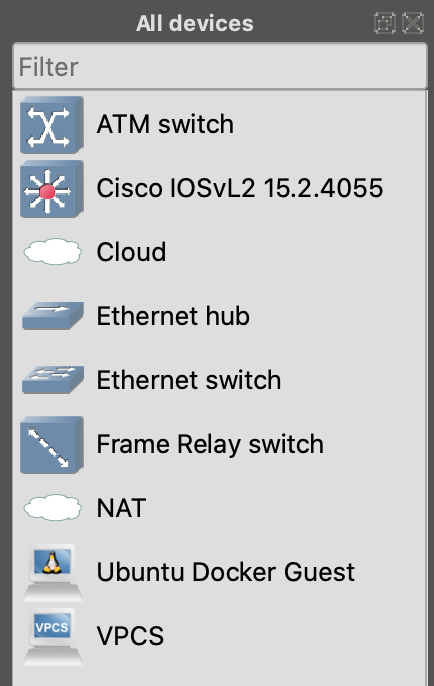
\includegraphics[width=.8\linewidth]{gns3-appliances-dock}
  \captionof{figure}{The appliances dock}
  \label{fig:gns3-appliances-dock}
\end{minipage}%
\begin{minipage}{.6\textwidth}
  \centering
  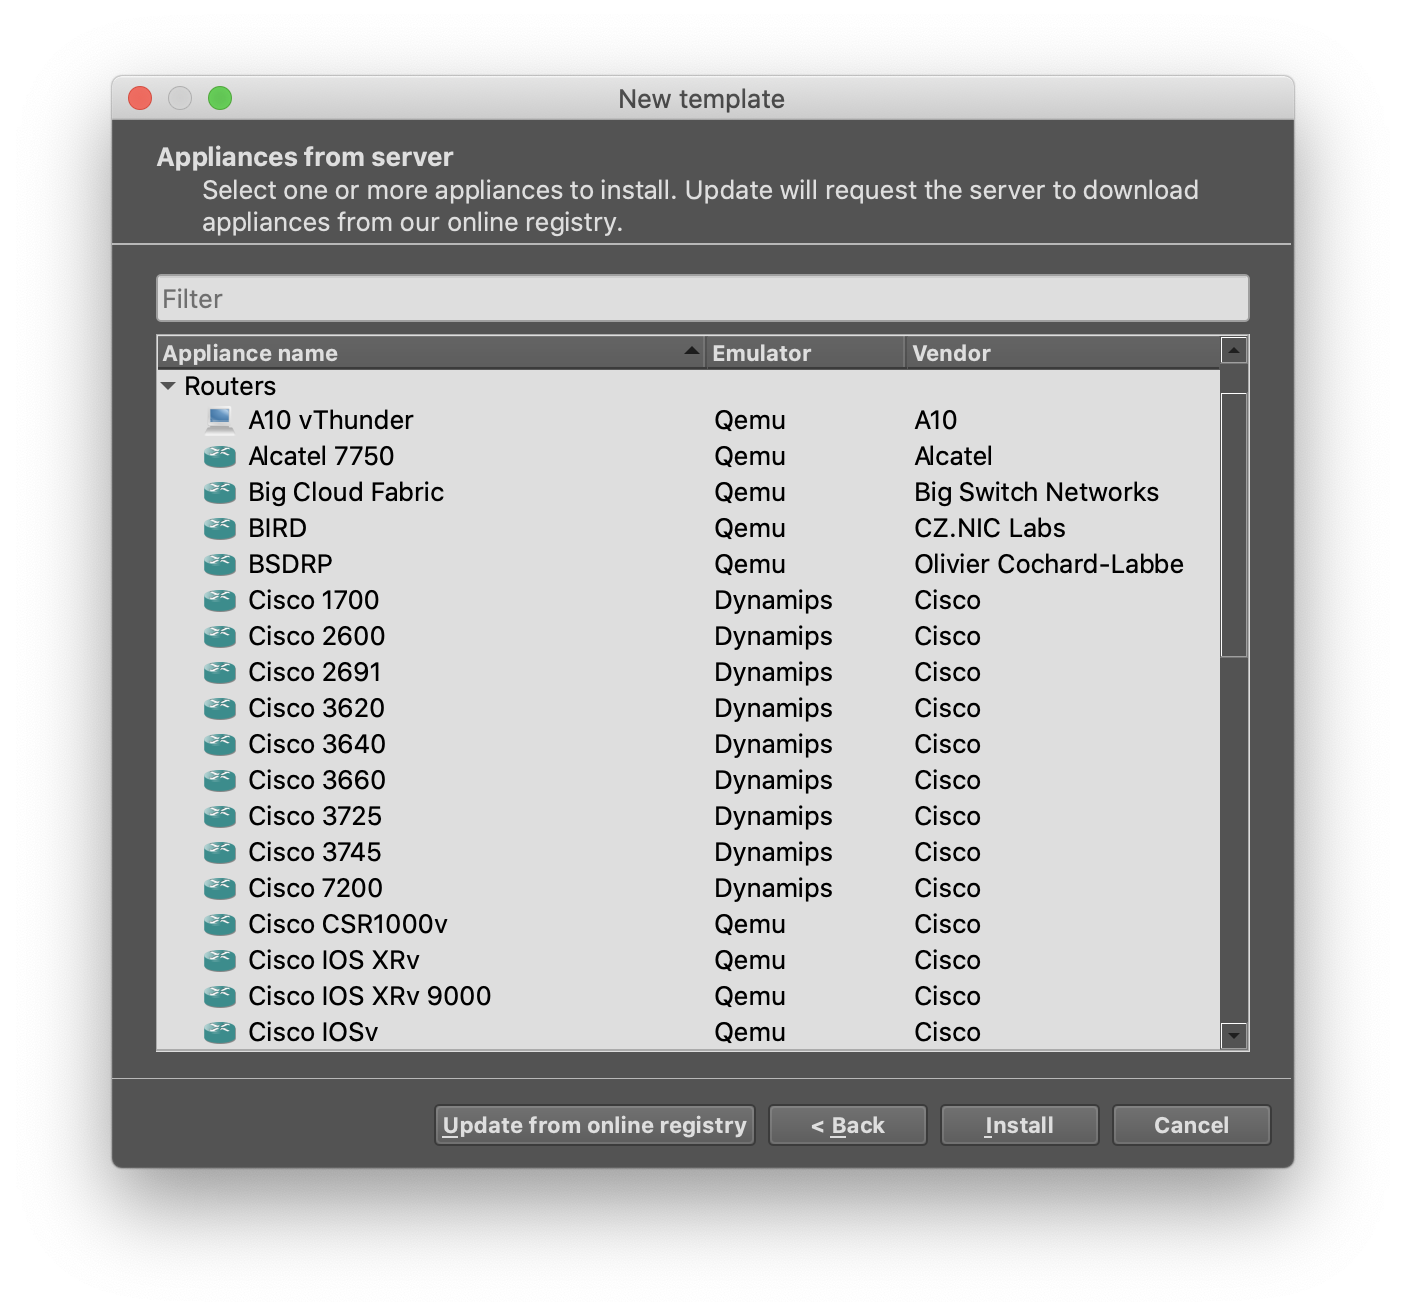
\includegraphics[width=.95\linewidth]{gns3-appliances-from-server-routers}
  \captionof{figure}{Some available router templates}
  \label{fig:gns3-appliances-from-server-routers}
\end{minipage}
\end{figure}


Deliberately, \emph{commercial} vendors of hardware, whose emulation is supported by GNS3, other than Cisco are excluded from this case-study for the following reasons:

\begin{enumerate}
  \item There isn't as near as many documentation and references in the literature, the web, or academic material for it as there is for Cisco.
  \item To narrow the scope of the investigation and this document, as the (again, commercial) network gear in laboratory used for the case study, FCT/NOVA's, is exclusively Cisco.
\end{enumerate}

Thus, this section is not intended to be exhaustive, or even less complete, in the sense of covering all the means GNS3 supplies out-of-the-box to emulate possible nodes in topologies.

\subsection{Dynamips and Legacy Cisco Routers}
\label{subsec:gns3dynamipslegacy}

GNS3 was initially built to leverage the Dynamips emulator~\cite{thebookofgns3}.
This program is a pure hardware emulator for MIPS processors geared towards full-compatibility with a series of Cisco (now legacy) router hardware models, namely the 1700, 2600, 3600, 3700, and 7200 series. % TODO add 'MIPS' to gls
Not only it the emulator is able to execute MIPS machine-level instructions, it also is able to boot real, uncompressed images for the real hardware and provide virtual interfaces and slots for modules corresponding to those in the physical counterparts.

Dynamips does not support Cisco Catalyst layer-2 switches, only the aforementioned layer-3 modular routers.
All it offers for switching capabilities is, for some models, the ability to insert a module, called EtherSwitch, which provides 16 switched ports to the routers, and allows for \emph{some} experiments with the switching capabilities (VLANs, STP) to be made.
However, \cite{thebookofgns3}, which has a lengthy reference on using Dynamips, its advantages and disadvantages is clear in stating that it isn't without its limitations, which comprehensively listed in this reference.

In a video published in the already mentioned semi-official GNS3 YouTube channel, the software's creator Jeremy Grossmann clearly states that Dynamips is not recommended for production these days, since, as will be seen later, more modern and maintainable solutions exist. At the same time, the GNS3 creator and lead developer also states that there are not plans to remove Dynamips support in upcoming versions~\cite{ytdynamipsvpcs}.

That is not say that, if no ``advanced'' features are intended, Dynamips, whose processes are extremely light compared to most of the alternatives, isn't the right solution, if the user or institution has access to licensed legacy IOS images. % TODO add ref to the performance part

\subsection{QEMU and Cisco IOSv}
\label{subsec:gns3ciscoiosv}

Another way to have Cisco gear inside a topology is using Cisco IOSv images, provided by the vendor itself as part of having access to their proprietary Virtual Internet Routing Lab (VIRL)~\cite{ciscovirl}.
IOSv, which concretely are IOSvL2 and IOSvL3 (standing for layer-2 and layer-3, respectively) are described as ``an implementation of Cisco IOS running as a full virtual machine on a hypervisor''~\cite{ciscoiosvinfo}.

On GNS3 this is accomplished via QEMU, a free and open source, general purpose emulator~\cite{qemu}.
In particular, the way GNS3 uses QEMU is not as an emulator, but as a wrapper for KVM~\cite{whatiskvm}, which ensures extremely good virtualized performance, though naturally limited to the resources of the hypervisor machine:
\begin{displayquote}
Run KVM and Xen virtual machines with near native performance.\footnote{\url{https://www.qemu.org}}
\end{displayquote}

When an appliance for IOSv is added to a GNS3 setup using the template, a virtual disk image is provided and uploaded to the compute node.
It is then used for spinning up \glspl{vm} with virtual interfaces running the operating system provided in the image. % TODO make this an acr statement

\subsection{Guests and Other Appliances}
\label{subsec:gns3guestsappliances}

``Guest''s is how GNS3 refers, on its interface, to hosts that can be added in topologies.
Here, host is meant in a conventional way, as what can be simply referred to as ``PCs,'' ``servers,'' or ``clients.''
GNS3 also supports other special end-devices, which are not explored in this dissertation, such as the \gls{nat} or \emph{cloud} nodes.

A fresh install of GNS3 comes with only one guest appliance installed, VPCS.
This is a kind of simulated PC, developed by the GNS3 project\footnote{\url{https://github.com/GNS3/vpcs}} as a way to provide to GNS3's usable nodes, capable of transmitting and receiving network traffic through a virtual interface, via tools like \texttt{ping}.
Although the traffic it generates and receives is ``real,'' and other nodes' interconnected to VPCS instances are not aware that it does not come from the usual applications on a host running a full-blown operating system, it doesn't have a kernel or possibility to run software over it.
A running VPCS node is simply a process that provides a virtual network interface and has a simple command-line interface to which the GNS3 user can \texttt{telnet}.

An advantage of these nodes is that they consume minimal resources, thus a topology can have a large quantity of them, and still allow to test topologies by checking connectivity on a variety of (potentially complex) scenarios.
They were especially useful on previous versions of GNS3, when the only way to have virtual hosts running full operating systems on GNS3 topologies---and, through it, test more advanced scenarios, using real-life software tools---, was to orchestrate heavy VirtualBox or VMware Workstation \glspl{vm}, which are heavy, take time to boot, and its cost increases constantly with the number of instances.

Since version 2.1, though, GNS3 supports appliances based on Docker containers.\footnote{Only on compute nodes running Linux}
These are very lightweight and, excluding the resources consumed by the \texttt{dockerd} process (which runs only once on the host and still doesn't compare to one full-blown \gls{vm}), each live container isn't noticeable heavier than a VPCS process, while still providing a real UNIX shell and possibility to run potentially any GNU/Linux-compatible application.  % TODO confirmar (e citar)!!!
\begin{figure}
  \centering
  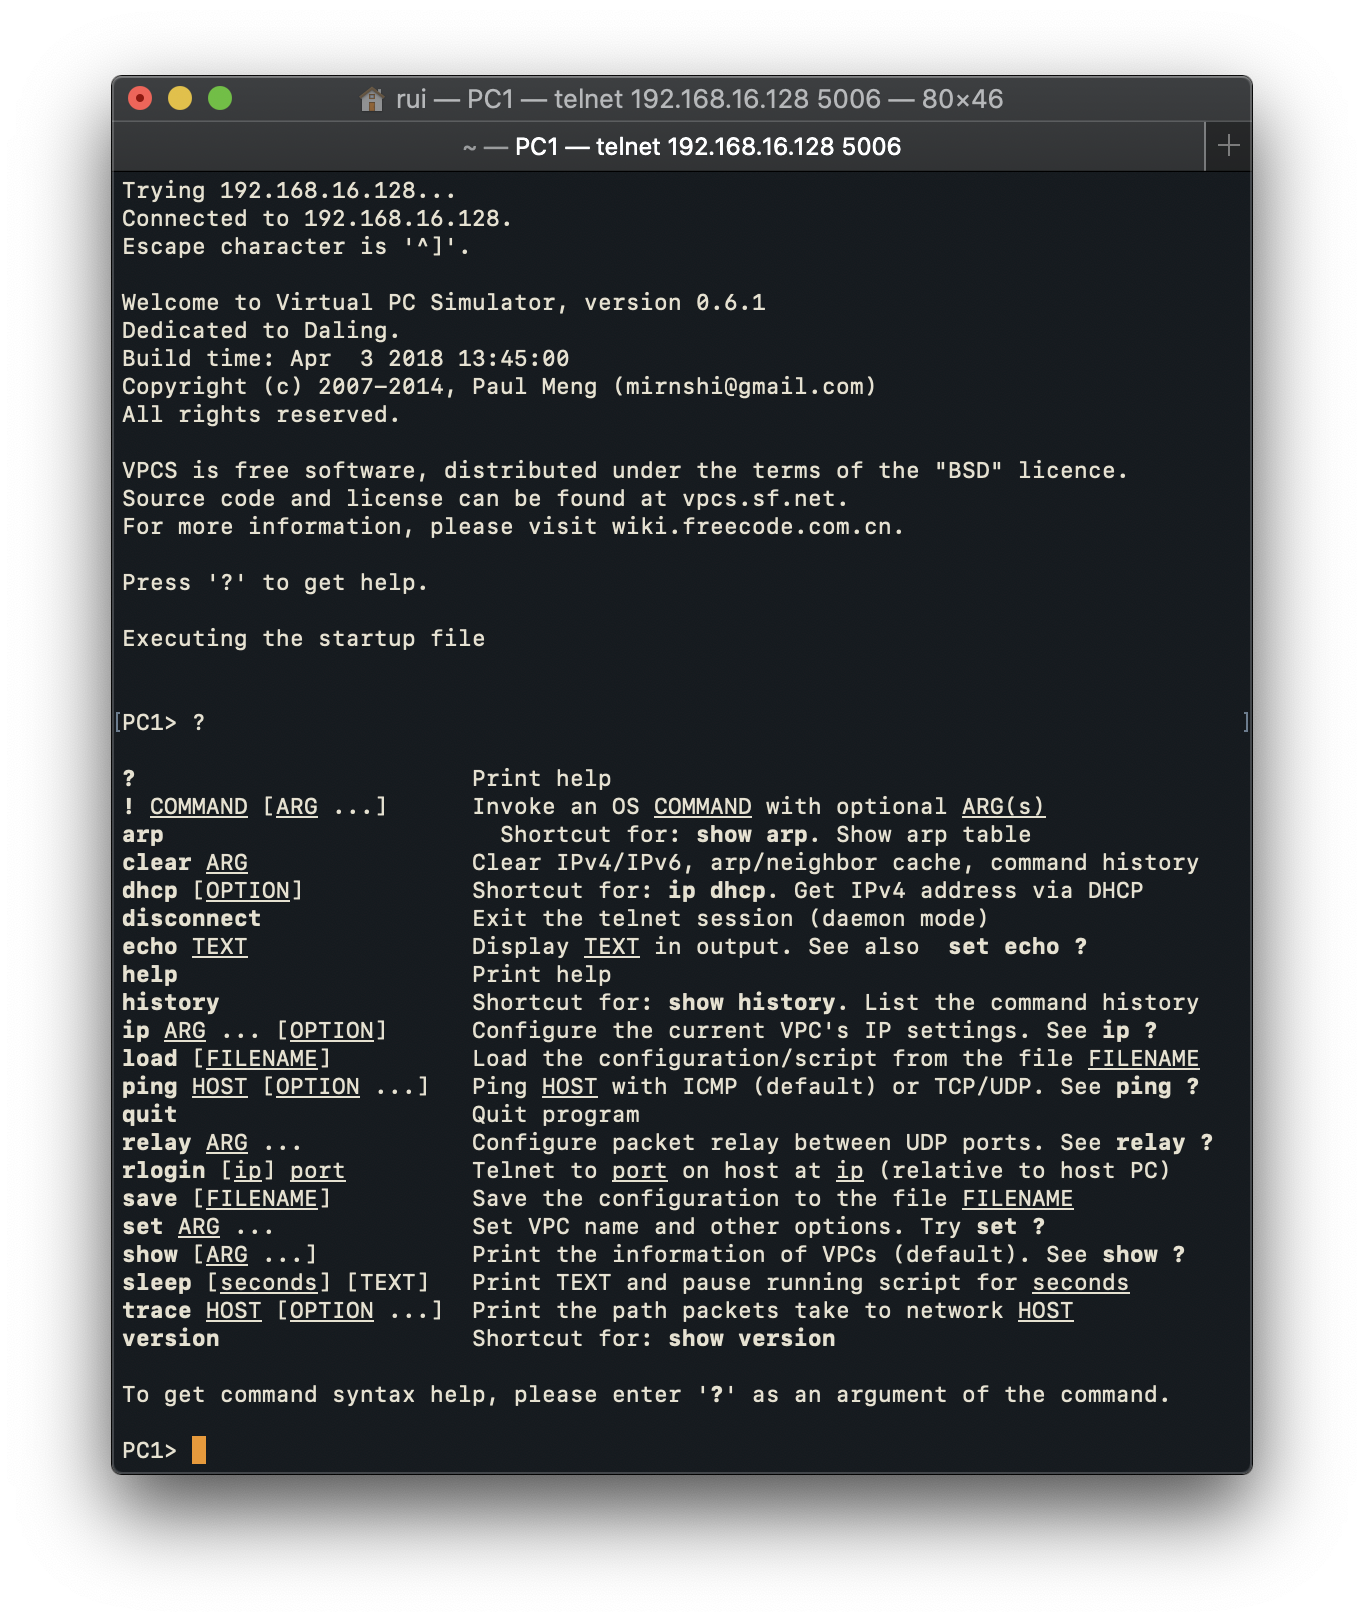
\includegraphics[width=0.6\textwidth]{gns3-vpcs-cli-help}
  \caption{A telnet session showing VPCS's list of commands}
  \label{fig:gns3-vpcs-cli-help}
\end{figure}

Due to this reason, the GNS3 project is recommending users to progressively stop using VPCS nodes and move towards Docker~\cite{ytdynamipsvpcs}.

The experiences carried out for this dissertation use exclusively Docker containers as guests.

\subsection{Links}
\label{subsec:links}

A crucial part, and arguably the only element common to really \emph{any} GNS3 topology, is the emulation of data links.
For any two nodes to communicate, their \gls{nic} must be connected through a ``pipe,'' through which bits can flow in two directions.
GNS3 maintains a program, with an independent code base and which can be used independently, outside GNS3, called ubridge (in some places stylized as uBridge).\footnote{\url{https://github.com/GNS3/ubridge}}
This program is the implementation of each of the straight lines that the user can draw on the canvas, clicking on two nodes, one after the other, and selecting the interfaces on each of them, to where the link is connected, reminding of a physical cable plugged on each free Ethernet port.

A deep study of ubridge wasn't carried out to know the implementation details.
What is practically observable is that, for each link, for each running interface on both of its ends (0, 1, or 2, depending on the status of the nodes), a user-level \texttt{ubridge} process exists on the compute's OS.

These processes listen on the virtual/software interface they were plugged in and encapsulate the traffic in UDP packets and send them through the compute's host OS network stack to the \texttt{ubridge} process on the other end of the logical link (it may or may not be running on the same compute). % TODO put UDP on glossary/acronyms
Conversely, they receive UDP datagrams, de-encapsulate the traffic inside them, and ``inject'' them back on the virtual interface they are attached to.

% <IF TIME, INVESTIGATE AND BRIEFLY DESCRIBE HOW THIS ``ATTACHMENT'' WORKS> % TODO <- ver!

ubridge is known to provide functionality of configuring simulating packet loss (by frequency or percentage), time delay in packet delivery, corruption of a fraction of the packets, or a Berkeley Packet Filter (for filtering out packets matching an expression)~\cite{ubridgereadme}.

% end of section gns3emulating
